\section{Mutua esclusione e sincronizzazione}\label{capitolo7}
Come prima cosa dobbiamo distinguere tra \emph{muta esclusione}, ovvero l'insieme di meccanismi che svolgono la funzione di proteggere dei dati condivisi da degli accessi concorrenti, e \emph{sincronizzazione} che sono i meccanismi che permettono la coordinazione tra threads e processi che vengono eseguiti in parallelo. I meccanismi di sincronizzazione sono costruiti attorno a quelli di mutua esclusione.\\
Il problema principale quando parliamo di multithread o multi-processi è quello di ottenere un risultato deterministico, ovvero in esecuzioni differenti ottenere esattamente lo stesso risultato pur avendo inevitabilmente un accesso alle variabili in modo sempre diverso. Per ottenere questo risultato è necessario sfruttare delle tecniche di sincronizzazione che possono essere sia hardware che software.\\
Un aspetto fondamentale della sincronizzazione è che un processo o un thread deve essere in grado di eseguire determinate operazioni su delle determinate strutture dati senza la possibilità di essere interrotto; tale sequenza di operazioni è denominata \emph{sezione critica}.\\
I meccanismi di sincronizzazione sono costruiti a livello utente tramite delle procedure software che sfruttano istruzioni di sincronizzazione fornite dallo hardware. Queste istruzioni devono permettere la lettura e la modifica di aree di memoria in modo \emph{atomico} ovvero senza essere interrotte. Esistono diverse soluzioni per implementare la mutua esclusione ad esempio l'uso della coppia \texttt{lock}-\texttt{unlock}, la sincronizzazione punto a punto tramite \emph{flags} o la sincronizzazione globale tramite barriere.\\
Le principali caratteristiche che contraddistinguono un metodo di sincronizzazione da un altro sono principalmente tre:
\begin{description}
\item[Metodo di acquisizione:] ovvero i modi in cui il processo tenta di acquisire i diritti per la sincronizzazione.
\item[Algoritmi di waiting:] i metodi utilizzati dal processo per attendere che la sincronizzazione sia disponibile.
\item[Metodi di rilascio:] i modi in cui un processo permette agli altri processi di procedere alla sincronizzazione.
\end{description}
Per quanto riguarda gli algoritmi si attesa esistono due alternative principali, la prima è quella di \emph{busy-waiting} nel quale il processo attende tramite un ciclo che la variabile di sincronizzazione cambi il suo valore, nel secondo caso la soluzione è \emph{bloccante} e in questo caso quando il processo entra in fase di attesa si blocca e lascia il processore ad un altro processo.
\subsection{Mutua esclusione}
La mutua esclusione è composta da due operandi \emph{lock} e \emph{unlock} i quali sono molto efficaci in caso di livelli di contesa delle risorse molto basso ma diventano molto inefficienti quando questi livelli di contesa si alzano. Esaminiamo due processi $P_j$ e $P_k$ i quali sono eseguiti su due nodi distinti e modificano entrambi la stessa struttura dati $D$ le due modifiche non hanno precedenza ma devono avvenire in modo atomico. Lo schema di questo esempio è mostrato in \figurename\,\ref{fig:lockexemp}
\begin{figure}[htb]
\centering
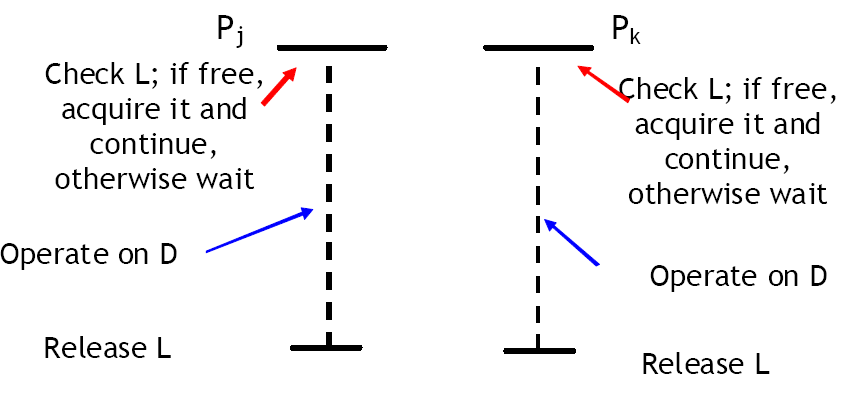
\includegraphics[scale=0.5]{img/lockexemp.png}
\caption{Esempio di due processi che sfruttano il lock}\label{fig:lockexemp}
\end{figure}
Un'altra primitiva molto comune è quella dell'\emph{atomic exchange} la quale si incarica di effettuare lo scambio di un valore nei registri con uno in memoria e viceversa. Tale metodo può essere utilizzato per implementare un semplice lock:
\begin{enumerate}
\item Prendiamo in considerazione un registro nel quale se il valore è 0 allora il lock è libero se invece il valore è 1 il lock non è disponibile
\item Un processo prova ad acquisire un lock su di una risorsa scambiando il valore in memoria con il valore 1 contenuto in un registro.
\item Il valore scambiato risulterà essere 1 se il lock è già stato scambiato, 0 altrimenti.
\end{enumerate}
Due soluzioni più recenti per implementare dei meccanismi di lock sono \emph{load linked} e la \emph{store conditional}. Se un contenuto di una memoria puntato da una \emph{load linked} cambia prima che la \emph{store conditional} effettui la scrittura allora la scrittura fallisce; ovvero se tra una load e una store il processore effettua un \emph{cambio di contesto} allora la store fallisce.
\subsection{Dalle primitive di sincronizzazione ai metodi di sincronizzazione}
Utilizzando le primitive di sincronizzazione è possibile costruire dei meccanismi che implementano la sincronizzazione a livello software. Il primo che analizziamo è lo \emph{spin lock} un meccanismo che utilizza le operazioni atomiche. In questo meccanismo un processo tenta di acquisire un lock in modo continuo tramite un loop fino a quando non ha successo. Tale meccanismo è utilizzato soprattutto quando il programmatore si aspetta che i lock siano trattenuti per un breve periodo di tempo e siano richiesti con scarsa frequenza. Un esempio del funzionamento di questo meccanismo è mostrato in \figurename\,\ref{fig:spinlock}
\begin{figure}[htb]
\centering
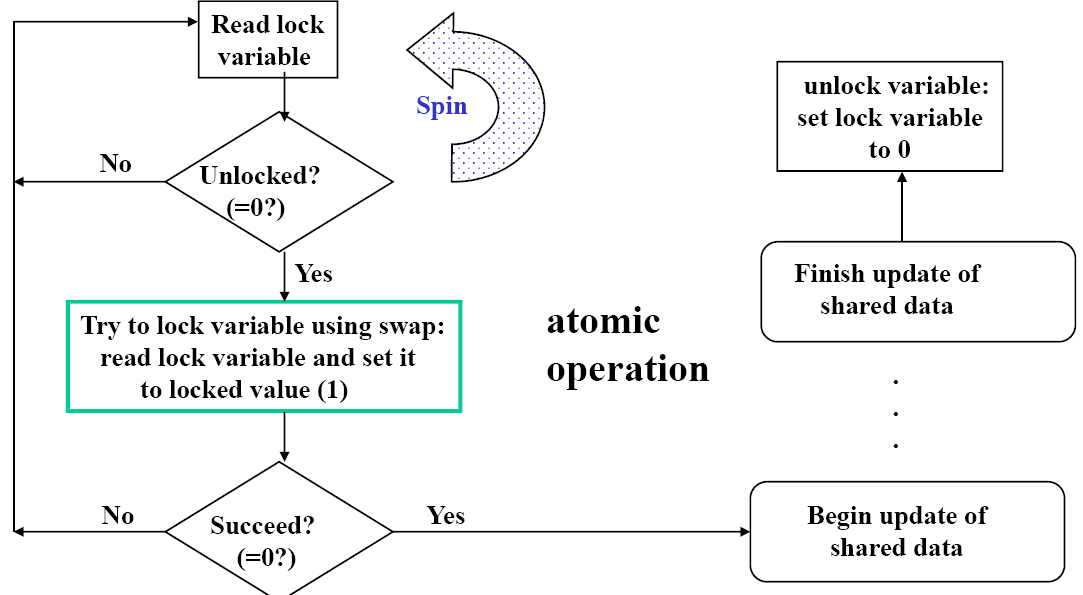
\includegraphics[scale=0.5]{img/spinlock.png}
\caption{Diagramma di flusso dello spin lock}\label{fig:spinlock}
\end{figure}
Un meccanismo di sincronizzazione ideale deve mantenere alcune caratteristiche per essere performante:
\begin{description}
\item[Bassa latenza:] ovvero il tempo necessario per acquisire un lock da parte di un processo quando questo è libero e nessun altro processo sta tentando di acquisirlo deve essere basso.
\item[Basso traffico:] se molti processi stanno tentando di acquisire uno stesso lock contemporaneamente essi lo devono ottenere in sequenza generando un traffico sul bus di dimensioni ridotte.
\item[Scalabilità]
\item[Basso costo di memoria]
\end{description}
Lo \emph{spin lock} tuttavia non rispetta molte di queste caratteristiche, infatti la latenza è bassa solo nel caso in cui uno stesso processo acquisisce il lock molte volte in successione, in caso di competizione per l'acquisizione del lock si genera molto traffico sul bus è difficilmente scalabile con l'aumentare dei processi.\\
Un altro meccanismo di sincronizzazione è quello del \emph{barrier} utilizzato soprattutto nel caso di loop paralleli. Tale meccanismo è di tipo globale e si applica ad un numero predefinito di processi \emph{p}. Per implementare tale meccanismo si utilizzano i lock, i contatori condivisi e le flags.
Per analizzare il funzionamento dell'algoritmo introduciamo l'esempio di un piccolo videogioco nel quale i frame vengono prima preparati e poi mostrati. Il codice di esempio che mostra il funzionamento è il seguente:
\begin{verbatim}
while (true) {
    frame.prepare();
    frame.display();
}
\end{verbatim}
è possibile ottimizzare il processo dividendo il processo in due thread il primo che disegna il frame e il secondo che prepara il successivo come mostrato in \figurename\,\ref{fig:barrierexemp}
\begin{figure}[htb]
\centering
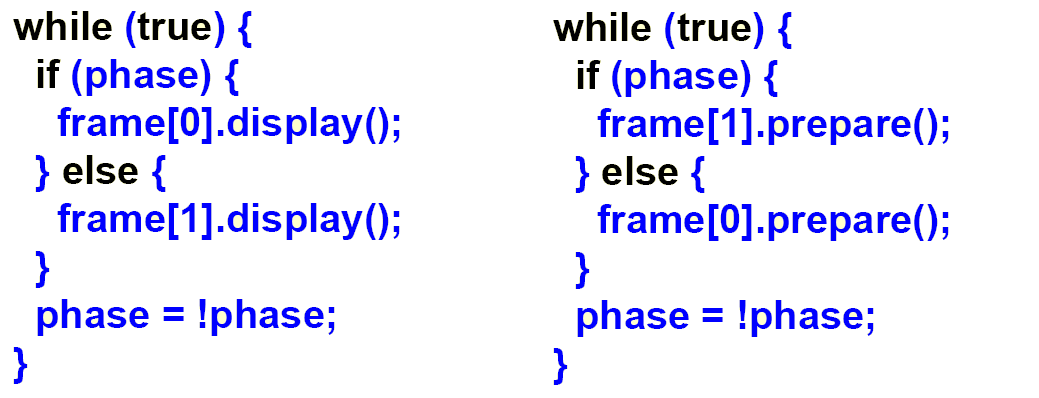
\includegraphics[scale=0.4]{img/barrierexemp.png}
\caption{Esempio di parallelizzazione del codice precedente}\label{fig:barrierexemp}
\end{figure}
Tuttavia possono sorgere alcuni problemi come un processo che si sveglia in ritardo e non prepara il frame in tempo come si mostra in \figurename\,\ref{fig:barrierfail} per questo motivo è stato introdotto il meccanismo del barrier.
\begin{figure}[htb]
\centering
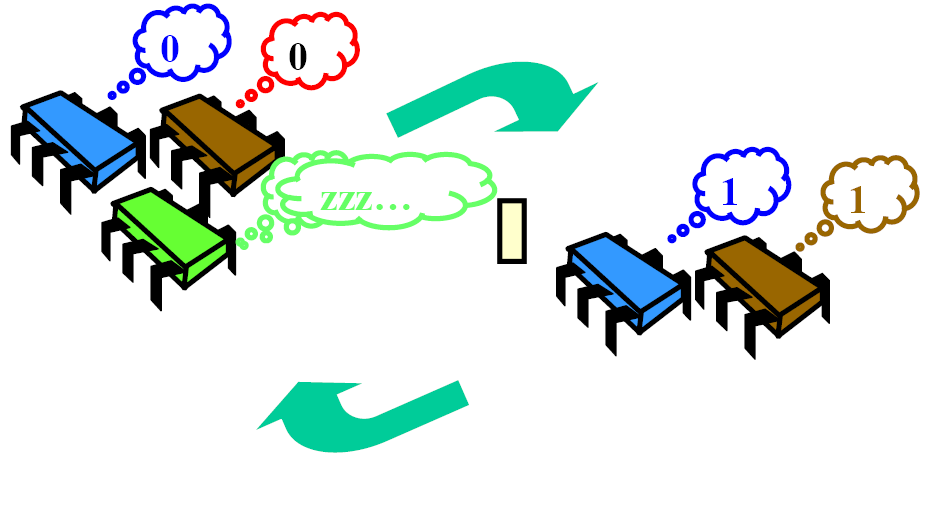
\includegraphics[scale=0.5]{img/barrierfail.png}
\caption{}\label{fig:barrierfail}
\end{figure}
Il meccanismo del barrier centralizzato mantiene il numero dei processi che arrivano alla barriera, per ogni processo che arriva un contatore viene incrementato, tale incremento deve essere atomico. Dopo ogni incremento il processo controlla se il numero dei processi $p$ coincide con quello del contatore, in caso negativo attende, in caso affermativo comunica agli altri processi tramite dei flag che la loro attesa è finita. Un esempio di implementazione di un sistema di barrier è mostrato in \figurename\,\ref{fig:barrierimp}
\begin{figure}[htb]
\centering
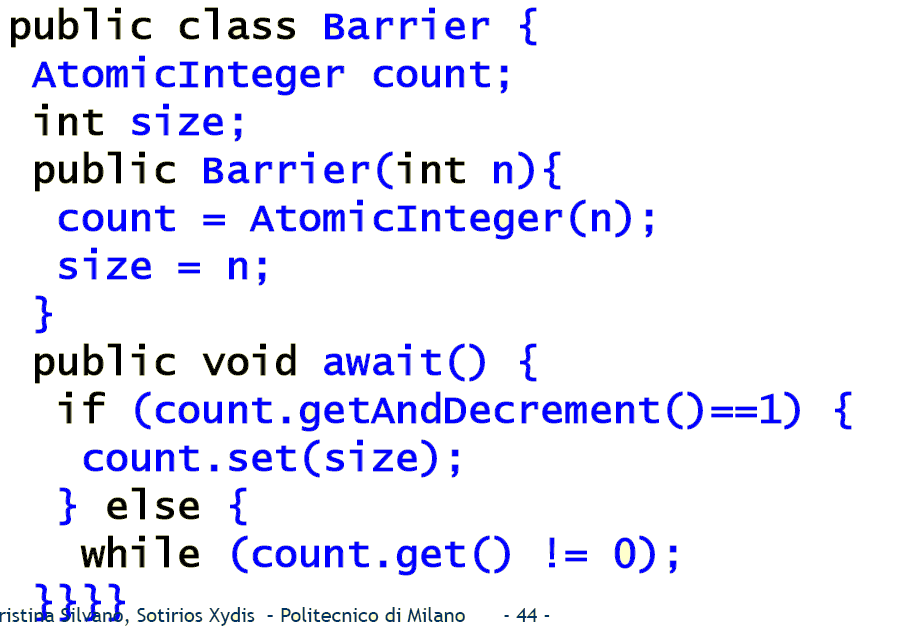
\includegraphics[scale=0.5]{img/barrierimp.png}
\caption{Implementazione di un sistema di barrier}\label{fig:barrierimp}
\end{figure}
Il problema di questo sistema è che risulta impossibile riutilizzare il barrier, per risolvere tale inconveniente si è pensato ad un sistema denominato \emph{sense-reversing barrier}. Ogni oggetto barrier contiene, diversamente dal caso precedente, un campo booleano che indica il senso dell'esecuzione corrente. Ogni thread mantiene traccia del senso corrente dell'esecuzione quando un thread raggiunge il barrier controlla se è l'ultimo thread e se lo è oltre a resettare il contatore inverte il senso dell'esecuzione, in caso contrario attende che il senso dell'esecuzione cambi; un esempio di questo meccanismo è mostrato in \figurename\,\ref{fig:barrierimp2}
\begin{figure}[htb]
\centering
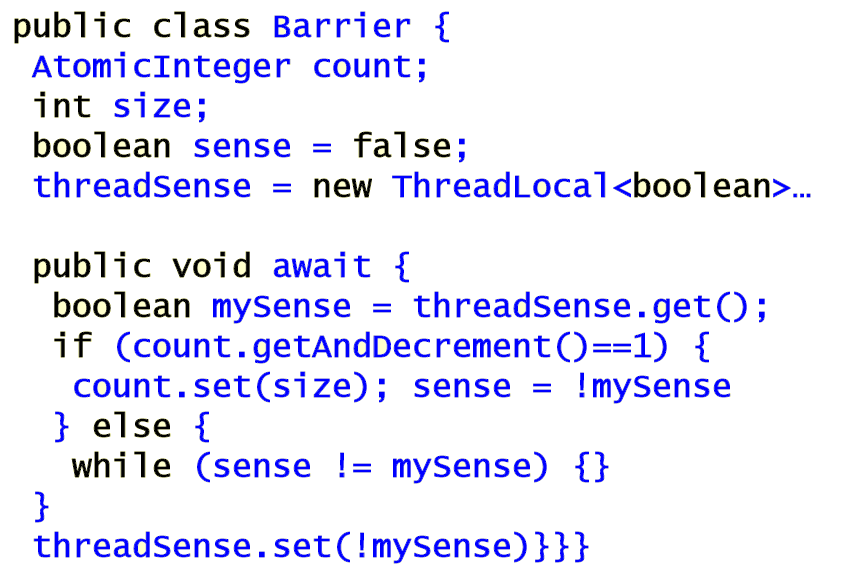
\includegraphics[scale=0.5]{img/barrierimp2.png}
\caption{Implementazione di un sistema di barrier con senso di esecuzione}\label{fig:barrierimp2}
\end{figure}